\section{Experiments}
\label{sec:experiments}

Experiments were conducted in the KITTI Road/Lane dataset, part of KITTI Vision Benchmarking Suite~\cite{KITTI}. The dataset  contains  images for road and lane estimation for the task of image segmentation. It consists of 289 training and 290 test RGB images, with the size of 1242 pixels width and 375 pixels height. The ground-truth is manually annotated for two different road types: (i) road, road area composing all lanes; and (ii) lane, lane the vehicle is currently driving on. It is important to notice that the ground-truth is only available for training set and the test evaluation should be performed using KITTI Server.

%\remEwai{What is the resolution of the images?} \remFeli{Done}

In this work, only the road ground-truths is used and the lane annotations are ignored. This dataset contains the same image with different ground-truths for lane and road estimation. Then, we prefer to use the road estimation and build the classifier on a binary problem~(road and background). The road type is divided in three different categories of road scenes, namely: (i) uu\_road, urban unmarked; (ii) um\_road, urban marked; and (ii) umm\_road, urban multiple marked lanes.  

%\remEwai{Should be good to show examples of images and groundtruths from the dataset} \remFeli{I think we won't have enought space in this paper} 

To increase the number of images in the training set, a data augmentation procedure is performed. The following transformations were applied: pepper/salt noise, horizontal flipping (mirror), contrast change, brightness change, noise shadow and random rain/snow. Procedures that would create undesired behavior, such as the road in the sky and distortions that would change the nature of the objects in the scene, such as cars and pedestrians were avoided. Augmentation procedures resulted in 2601 images, divided in 2080 samples for training and 521 samples for validation (about 20\%). 


\subsection{Experimental setup}
   
Our networks were built using using Keras \cite{chollet2015keras} with Tensorflow \cite{tensorflow2015-whitepaper}. We used a pre-trained VGG16 model to initialize the weights. Also, we use SGD optimization with learning rate set to 1e-3, decay of 5e-6 and momentum of 0.95. The default batch size contains 16 images. To fit the network and speed up the process, all images were reduce to 624 pixels width and 192 pixels height (about 50\%). Training experiments were performed in GeForce GTX 1080 8GB GPU.

The \textbf{SLO} network is composed of $n=5$ side-outputs, and the \textbf{ALO} network is composed of $n=13$ side-outputs. 
The operations to combine side-outputs are presented in the name of the methods. The merging operations \textbf{ADD}, \textbf{AVG} and \textbf{MAX} are available for both ALO and SLO methods.
As a baseline, we use the VGG16 network without any side-output but only the final output, called No Side Outputs~(\textbf{NSO}).

\subsection{Training results - Methods Comparison}

The first test was design to identify the best neural network and its best merging methods. We train all nets with all merging methods for 100 epochs to determine which one learns faster and achieves the best results. This conduct lead us to understand how layers can be easily combined to produce outputs with good precision.

Figure \ref{fig:validation_loss} presents the categorical cross-entropy loss curves obtained during the training phase for the proposed approaches. ALO networks appear to be more stable with a faster decay than NSO and all SLO approaches. Also, it is important to notice that NSO and SLO-MAX produce high instability in the learning course. On the other hand, ALO-AVG presents the best result for the test, followed by ALO-MAX and ALO-ADD merging strategies.

\begin{figure}
  \caption{Categorical Cross Entropy Validation Loss}
  %\remEwai{Only Pixel Error according to the text} \remFeli{Changed}
  \centering
    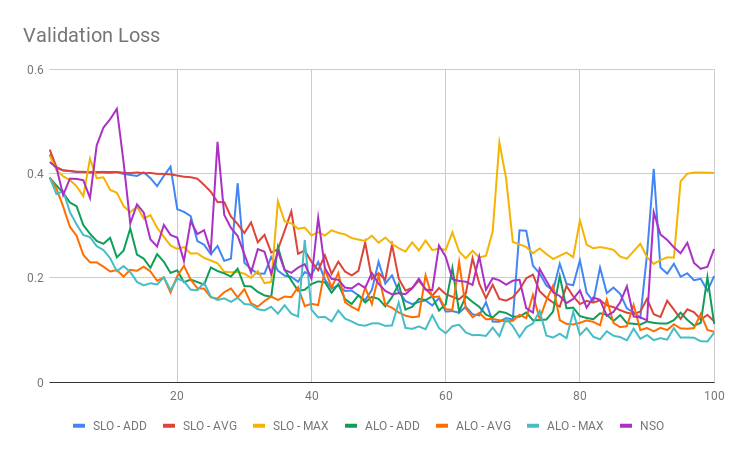
\includegraphics[width=1.\columnwidth]{figures/falreis/validation_loss.png}
  \label{fig:validation_loss}
\end{figure}

From previous graph, it is possible to conclude that ALO networks had superior and more desirable behavior than the SLO and NSO models. It is believed that these results are consequence of the considerably larger amount of side-outputs, which create more possibilities of interchangeability between confident values.

\subsection{Best results}

In order to improve the results, a new set of tests were performed using 500 training epochs. As some networks had a poor performance in the previous test and other tests with different parameters, we decided to evaluate only ALO network in this new round of tests. 

To measure the performance in our tests we use two different metrics. The first one is the well known categorical cross entropy accuracy. Also, we use an metric called pixel-error. This measure evaluates the number of pixels incorrectly classified over the total number of the pixels (number of wrong pixels). These two metrics are available in Figure \ref{fig:val_acc_500_epochs}.

\begin{figure*}
  \caption{Categorical Cross Entropy Validation Accuracy and Pixel-Error results for 500 epochs test set}
  \centering
  \begin{tabular}{ll}
    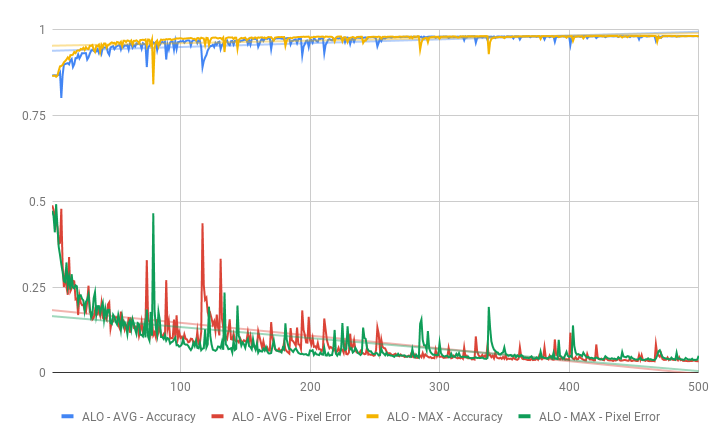
\includegraphics[width=1.\columnwidth]{figures/falreis/val_acc_500_epochs.png}
  
    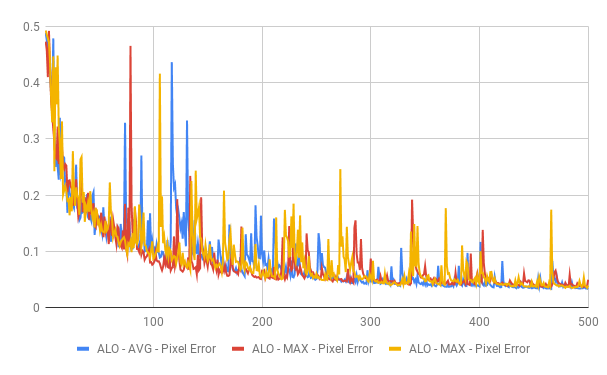
\includegraphics[width=1.\columnwidth]{figures/falreis/pixel_error_500_epochs.png}
  \end{tabular}%
  \label{fig:val_acc_500_epochs}
\end{figure*}

The best results of both metrics are quite similar for all networks. This indicates absence of a far better method to combine side-outputs. The best result for cross entropy validation metric is just \textbf{0.0009} above the worst one (0.983 for ALO-ADD and 0.9821 for ALO-AVG). For pixel-error, the best value is just \textbf{0.0040} above the worst one (0.0332 for ALO-AVG and 0.0372 for ALO-MAX).

Due to the similarity of the results, we will indicate the best method using the value of validation pixel-error metric. Also, AVG fusion method was also previous used in \cite{xie2015} and \cite{liu2017} to combine the results. For this criteria, ALO-AVG was defined as the best method of our training set.

\subsection{Post-processing using mathematical morphology}

%\remEwai{Insert reference to section IV that describes that post-processing. \cite{najman13} should go in section IV.} \remFeli{Partial Done}

After the training procedure, we create a post processing step to reduce possible noises in results proposition. For this, we used the mathematical morphology operation of Opening, as defined in Section \ref{ssec:post_processing}. This procedure removes small noises created by the foreground~(the road) in the background. 

The opening operation was applied using square structuring elements full of ones. We decided to use a set of kernels with sizes of $5\times5$, $7\times7$, $9\times9$, $11\times11$ and $13\times13$, sequentially applied into the image. This type of operation, although unusual, achieved the best results. It allowed that sections incorrectly classified by the network could be eliminated by the sequential thinning of noises in different shapes. The results also become more smooth with this procedure.

%\remEwai{I don't understand here. All the structuring elements are applied sequentially? which makes no sense since the opening by the largest structuring element is included in the opening by the smallest structuring element if I'm right. Or are they all tested independently? In this latter case, which size is finally retained?} \remFeli{Yes, sequencially. Although unusual, it removed incorrect classification better than small kernels alones. (Text changed for better explanation)}

A simple comparison of our procedure with the original network prediction is presented in Figure \ref{fig:post_processing_comp}. In this image, we selected an output result that clearly shows the benefits of mathematical morphology post processing. It is possible to see the removal of part of the noise in the far right of the image (\textit{white pixels}). The noise removal increases the confidence, as small variations in the results can lead to a potential problem, if used in a self-driving vehicle. 

\begin{figure}
  \caption{Comparison between ALO-AVG without post processing and ALO-AVG with post-processing with mathematical morphology. In the last picture, \textit{white} pixels represents desirable differences while \textit{red} pixels represents undesirable ones.}
  \centering
  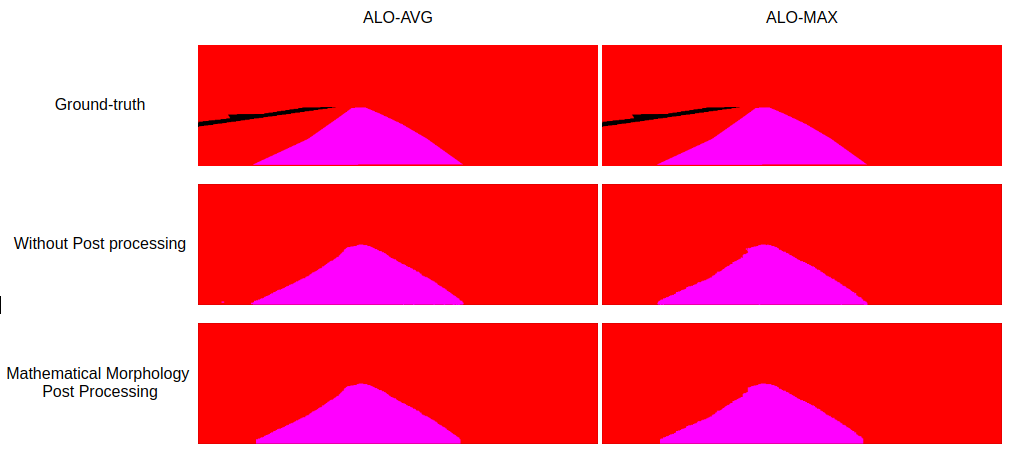
\includegraphics[width=1.\columnwidth]{figures/falreis/post_processing_comparison.png}
  \label{fig:post_processing_comp}
\end{figure}

A side effect of this method is the removal of some points that seems to fit correctly. This situation happens frequently in the base of the road proposition. In Figure \ref{fig:post_processing_comp}, it can be seen in the bottom left and the bottom right of the road (\textit{red pixels}).

\subsection{Side-outputs contribution in each merging strategy}
\label{ssec:merging_learn}

Each layer of each merging strategies learns in its particular way. The merging strategy influences how the networks learn. It is possible to see how each side-output learns and contributes to the final output in Figure \ref{fig:side_outputs}. To simplify the study of side-outputs, we decided to visualize only the last  output from each stage in \textbf{ALO} network, for our trained networks. To make the layers outputs easier to analyse, the images were  converted to black and white, where white pixels were classified as road and black pixels were classified as background.

%\remEwai{Not clear relatively to Fig. 2} \remFeli{Changed section. Removed Fig. 2 information.}

\begin{figure*}
  \caption{Side outputs for each merging strategy in ALO network.}
  \centering
  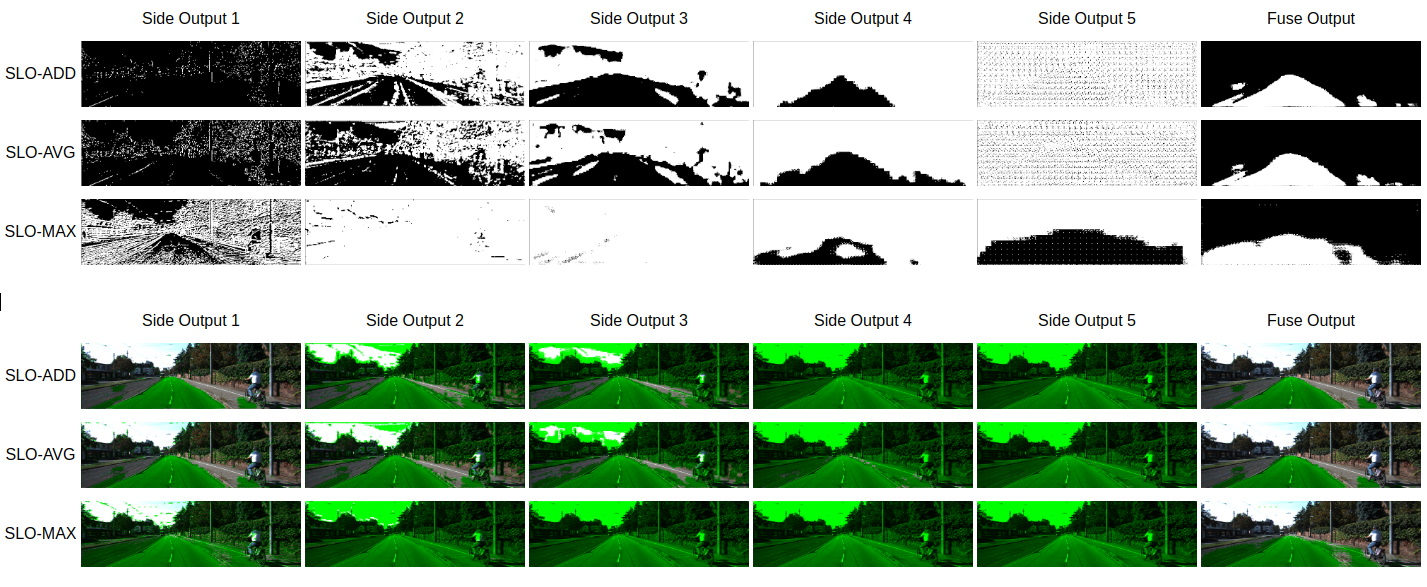
\includegraphics[width=1.0\textwidth]{figures/falreis/side_outputs.png}
  \label{fig:side_outputs}
\end{figure*}

%\remEwai{Fig. \ref{fig:side_outputs} is not so clear. Notation from the text should be reused: the side-output i what is denoted $\mathcal{H}_i$ (if I'm correctly understanding)} \remFeli{Changed. I don't know if it was clear enough. I'll think in how to improve it}

Figure \ref{fig:side_outputs} indicates that the first two stage side-outputs (outputs $\mathcal{H}_2$ and $\mathcal{H}_4$) does not produce significant information. Images are almost white, indicating that all pixels were classified as road. ALO-AVG and ALO-ADD third layer contains a clear separation between road pixel than non-road pixels. ALO-MAX's third layer, on the other hand, does not clearly separate road from non-road pixels. The results are pixelated and blur when compared with the original image.

Figure \ref{fig:side_outputs} also indicates that fourth stage side-output layer (output $\mathcal{H}_{10}$) clearly contains the best side-output for all ALO networks. The road marks are clearly visible, but with some noise. ALO-MAX contains a lot of noise, while ALO-ADD contains a few ones. The final stage side-output ($\mathcal{H}_{13}$) contains a lot of noise, with results far away worse than the previous layer. This possibly indicates that the layer was not able to correctly learn the information from the previous ones.

The fuse layer combine all side-outputs (including the ones not shown in Figure \ref{fig:side_outputs}) in order to predict. Despite poor results on some layers, the learning process adjusts itself so that even very few accurate results can be used by the model, similar to ensemble methods.

%\remEwai{= the proposition $Z$} \remEwai{? Not clear} \remEwai{merging layers = fuse layer?} \remFeli{Fixed. Text improved but I don't know if it is good enough. I don't know if I can cite ensemble methods.}

\subsection{Evaluation results and comparison with the state-of-the-art}

Reminding that the test evaluation could only be performed using KITTI Server, the metrics provided are maximum F1-measure~(MaxF), average precision~(AP), precision~(PRE), recall~(REC), false positive rate~(FPR) and false negative rate~(FNR). 

The server tests were performed using ALO-AVG method, the best one in the training process. To provide succint labels, we will use the name \textbf{ALO-AVG} for the regular approach and \textbf{ALO-AVG-MM} for the version with mathematical morphology post-processing. The results achieved  on the test set according to each category in the road scenes are presented in Table~\ref{tab:metrics}. 

\begin{comment}
{\color{As expected, the ALO-AVG-MM model performs better then the ALO-AVG in almost all the cases. red}It is also possible to notice that although the post-processing slightly improves the overall performance, it also increases the number of false negatives. This could be an indication that perhaps the applied kernel sizes are not adequate and are removing more of the foreground than desired.}
\end{comment}

If compared with the state-of-the-art~(called \textit{PLARD}, an anonymous submission on the KITTI Server platform \footnote{Results accessed in 2018-01-13}), the proposed method is comparable and sometimes superior, regarding the maximum F1-measure and the recall metrics. This is due to the fact that although the reported state-of-the-art on the dataset presents a superior average precision, it also almost always presents a higher rate of false positives and negatives. This indicates that the proposed methods are more precise in delineating the regions to be segmented.

\begin{table}
 \scriptsize
 \caption{KITTI benchmark evaluation results for each category}
  \begin{tabular}{{l}{c}{c}{c}{c}{c}{c}}
  
   \multicolumn{7}{l}{\textbf{um\_road}} \\
  \hline 
    Method & MaxF & AP & PRE & REC & FPR & FNR \\
  \hline
    \textit{SLO} & 96.92\% & 87.36\% & 94.47\% & \textbf{99.49\%} & 1.13\% & \textbf{0.51\%} \\
    \textit{SLO-mm} & \textbf{97.01}\% & \textbf{87.68\%} & \textbf{94.83\%} & 99.30\% & \textbf{1.05\%} & 0.70\% \\
    \textit{ALO}  & 96.39\% & 86.81\% & 93.87\% & 99.05\% & 1.25\% & 0.95\% \\
    \textit{ALO-mm} & 96.65\% & 87.51\% & 94.64\% & 98.74\% & 1.08\% & 1.26\% \\
    \textit{State-of-the-art} & \textbf{97.05\%}& \textbf{93.53\%} &\textbf{97.18\%} &\textbf{96.92\%} &	\textbf{1.28\%} &\textbf{3.08\%} \\
  \hline
  \multicolumn{7}{c}{} \\
  
  \multicolumn{7}{l}{\textbf{umm\_road}} \\
  \hline 
    Method & MaxF & AP & PRE & REC & FPR & FNR \\
  \hline
    \textit{SLO}  & 97.57\% & 89.44\% & 96.05\% & \textbf{99.15\%} & 1.24\% & \textbf{0.85\%} \\
    \textit{SLO-mm} & \textbf{97.61\%} & \textbf{89.67\%} & \textbf{96.30\%} & 98.97\% & \textbf{1.16\%} & 1.03\% \\
    \textit{ALO}  & 97.05\% & 88.83\% & 95.37\% & 98.78\% & 1.46\% & 1.22\% \\
    \textit{ALO-mm} & 97.21\% & 89.31\% & 95.90\% & 98.56\% & 1.29\% & 1.44\% \\
    \textit{State-of-the-art} & \textbf{97.77}\%&\textbf{ 95.64\%} &\textbf{97.75\%} &\textbf{97.79\%} &	\textbf{2.48\%} &\textbf{2.21\%} \\
  \hline
  \multicolumn{7}{c}{} \\
  
  \multicolumn{7}{l}{\textbf{uu\_road}} \\
  \hline 
    Method & MaxF & AP & PRE & REC & FPR & FNR \\
  \hline
    \textit{SLO}   & 95.16\% & \textbf{85.73\%} & 92.94\% & 97.49\% & 1.16\% & 2.51\% \\
    \textit{SLO-mm}  & \textbf{95.42\%} & 86.48\% & \textbf{93.77\%} & 97.13\% & \textbf{1.01\%} & 2.87\% \\
    \textit{ALO}   & 94.70\% & 84.87\% & 92.00\% & \textbf{97.56\%} & 1.33\% & \textbf{2.44\%} \\
    \textit{ALO-mm} & 95.20\% & 86.15\% & 93.40\% & 97.08\% & 1.08\% & 2.92\% \\
    \textit{State-of-the-art} & \textbf{95.95\%}& \textbf{95.25\%} &9\textbf{5.25\%} &\textbf{95.65\%} &	\textbf{1.21\%} &\textbf{4.35\%} \\
  \hline
  \multicolumn{7}{c}{} \\
  \end{tabular} 
  \label{tab:metrics}
\end{table}


A visual representation of ALO-AVG-MM predictions are presented in Figure \ref{fig:visual_representation}. This image shows the predictions marked (in green) over the road, to show the performance of our model. The generated subimages were provided by Kitti Evaluation Server, based in the generated binary map sent to the server.

\begin{figure}
  \caption{Visual representation of the results. The generated image was provided by Kitti Evaluation Server. Green pixels represents true positives, red pixels are false negatives and blue pixels are false positives.}
  \centering
  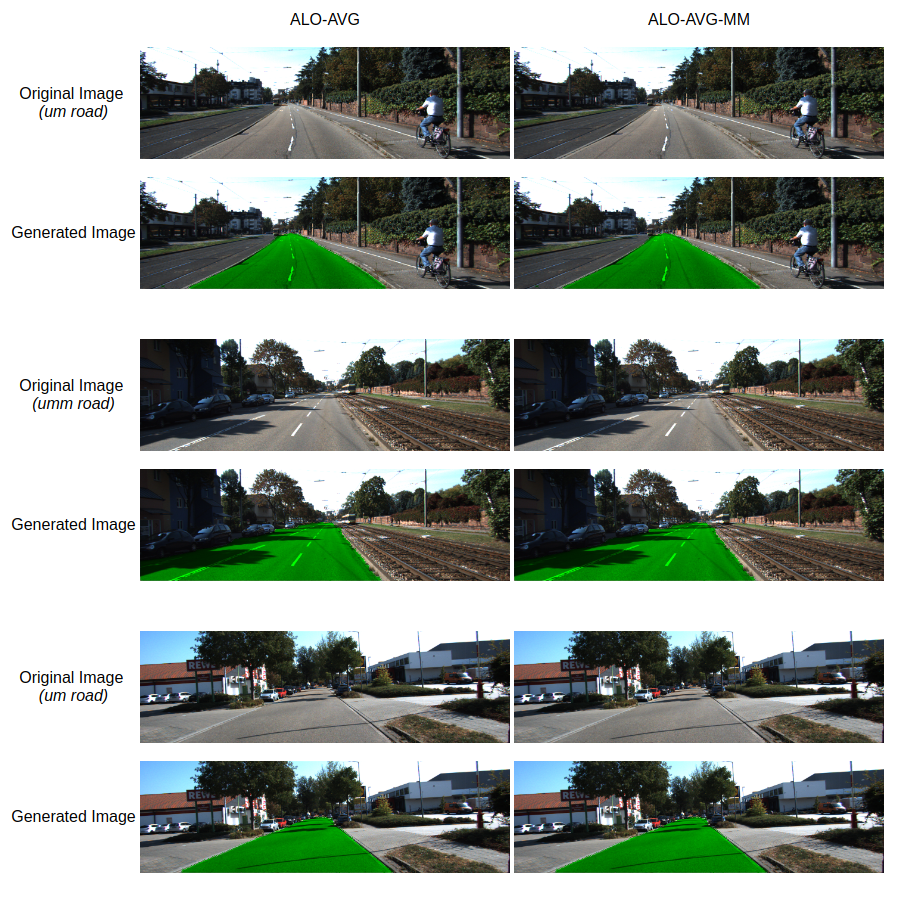
\includegraphics[width=1.\columnwidth]{figures/falreis/visual_representation.png}
  \label{fig:visual_representation}
\end{figure}
